\subsection{Visualisierungs-Phase} 
Nach vollständiger Beendigung der Scan-Phase ging es in der Entwicklung weiter mit der Visualisierungs-Phase. Die zuvor gespeicherten Objekte und 
deren Informationen werden dabei abgerufen und können jederzeit erneut visualisiert und im Raum platziert werden. Die folgende Darlegung der 
Frontend-Entwicklung der Visualisierungs-Phase gibt einen Einblick auf die Benutzeroberfläche dieser Phase und wie diese aufgebaut ist. Dadurch sind die 
zugrundeliegenden Informationen veranschaulicht, welche für die nachstehende Backend-Implementierung von Relevanz sind.   
\subsubsection{FrontEnd}
Bei der Visualisierungs-Phase gibt es prinzipiell eine Benutzeroberfläche, die diesen Use Case ausmacht. Unter eigentlicher Anwendung dieser Phase und 
deren \acs{GUI} befinden sich darüber hinaus weitere Benutzeroberflächen, die bereits in der Scan-Phase schon erläutert wurden. Darunter zum Beispiel 
die in Abbildung (\ref{pic:image_tracking}) zu entnehmende Markererkennungs-\acs{UI}, die ebenso Bestandteil der Visualisierungs-Phase ist. 
\\ 
Die primäre \acs{GUI} ist ähnlich zu der Benutzeroberfläche der Scan-Phase aufgebaut. Ein Fragment, welches das Livebild der Kamera repräsentiert, das 
sich über den ganzen Bildschirm erstreckt. Dadurch können die bereits in der Scan-Phase erstellten Objekte erneut angezeigt werden. Des Weiteren befinden 
sich auf dieser Oberfläche zwei Buttons, zum einen zur Navigation, um auf das Startmenü zu gelangen und zum anderen, um die Objekte von der Datenbank 
abzugreifen, rendern und auf dem Bildschirm anzeigen zu lassen. Diese befinden sich jeweils in der linken und rechten unteren Ecke des Bildschirms, wie 
der Abbildung \ref{pic:visual} zu entnehmen ist. 
\\ 
Da diese \acs{UI} nur als Ansicht der zu visualisierenden Objekte gedacht ist, stehen dem Nutzer nur eingeschränkt Interaktionen mit der Oberfläche zur 
Verfügung. Diese belaufen sich lediglich auf die zuvor genannten Buttons und die dynamisch erzeugten Schaltflächen der Objekte, um zu den einzelnen 
Darbietungen der Objekte mehrere Informationen zu erlangen. 
\begin{figure}[hbt!]
    \centering
    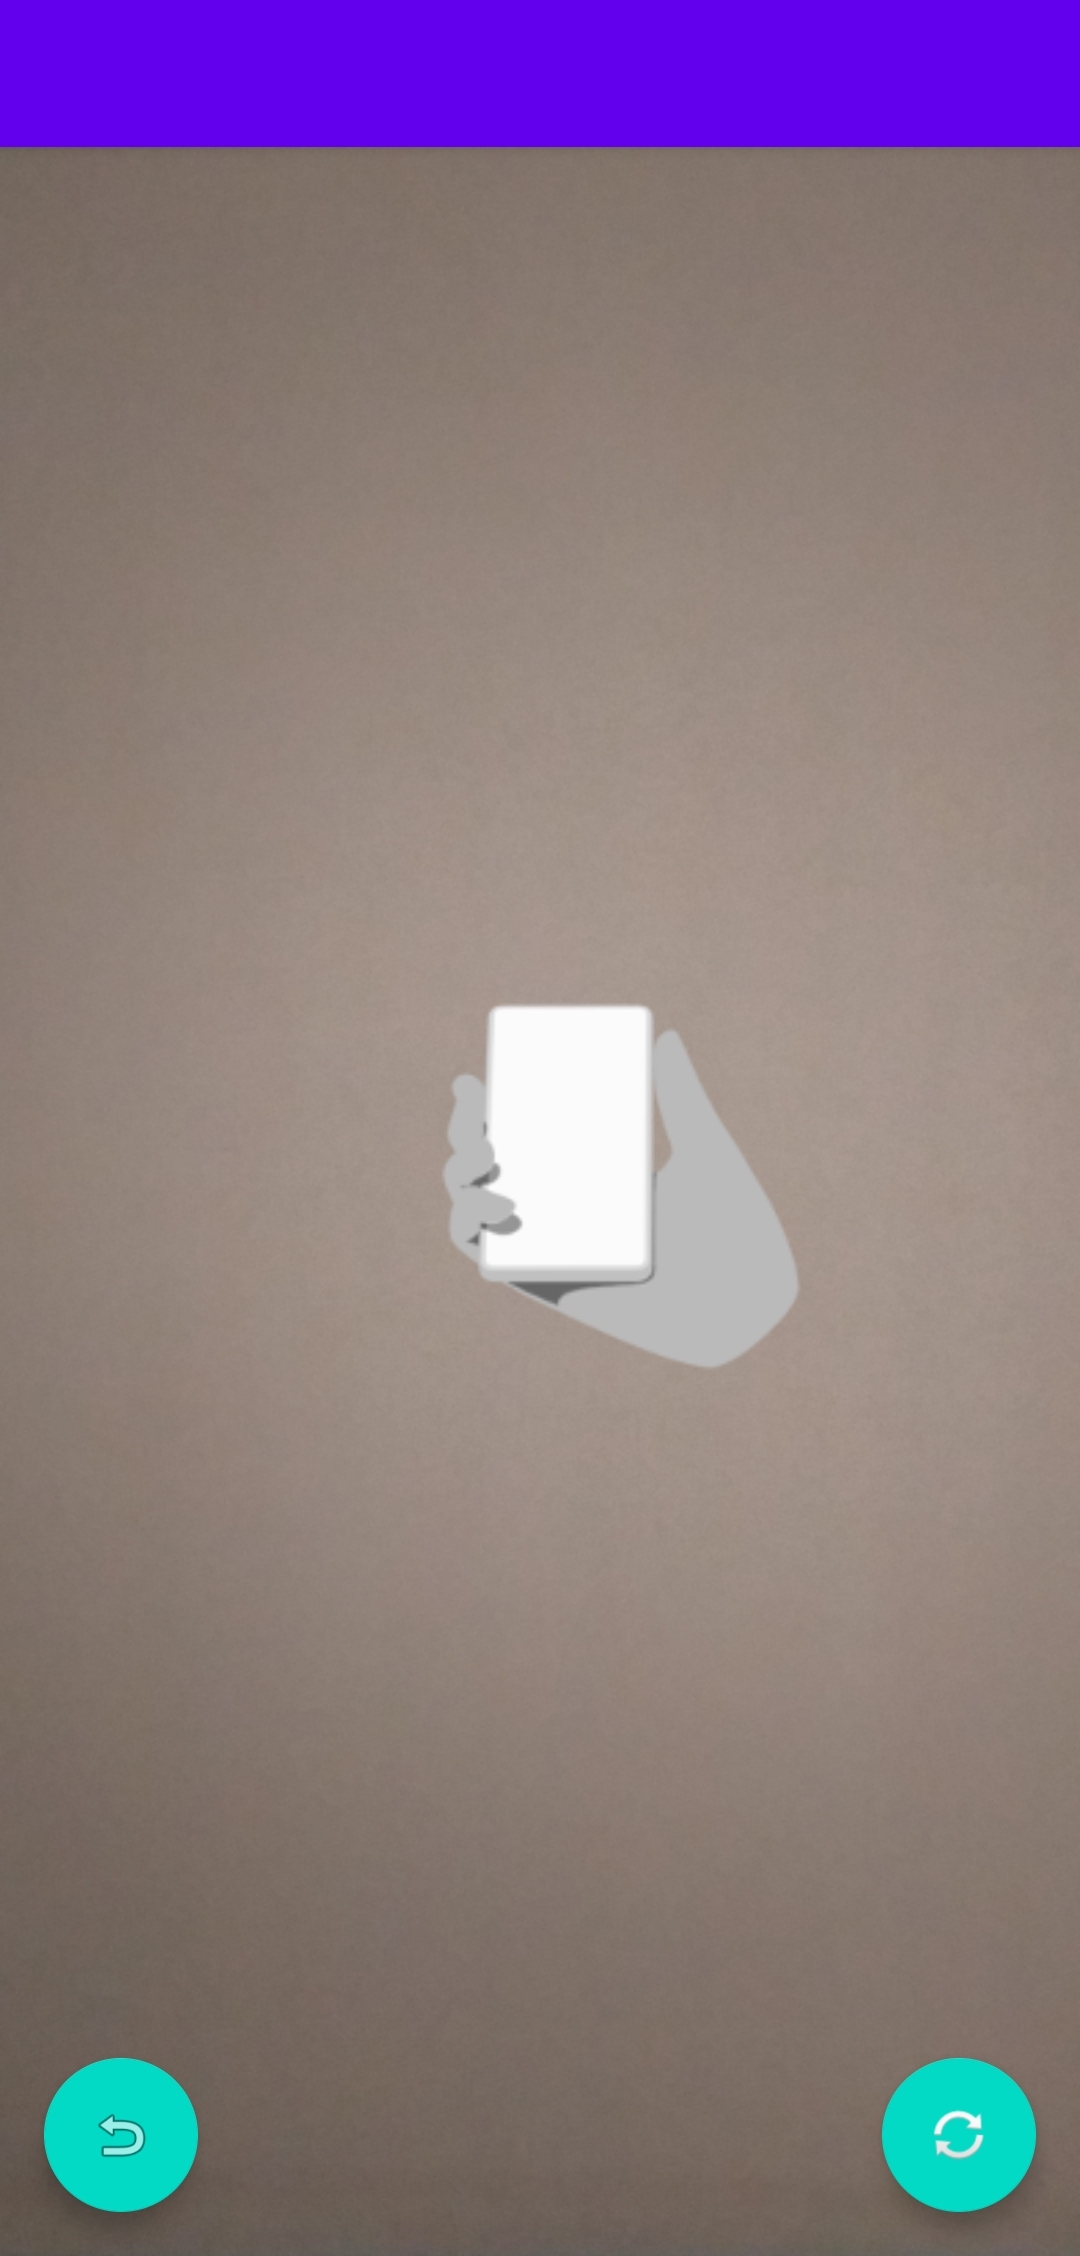
\includegraphics[width=10cm,height=7.5cm,keepaspectratio]{4Umsetzung/Bilder/visual-phase.jpg}
    \caption{Visualisierungs-Phase der Applikation}
    \label{pic:visual}
\end{figure} 
\\
Nun erfolgt die Beschreibung der Backend-Implementierung und Einblicke in die Programmierung der Visualisierungs-Phase werden gewährleistet. 
\subsubsection{BackEnd}
Nachdem das Problem der variablen Startposition in der Implementierung der Scan-Phase umgangen war, konnte die Visualisierungs-Phase entwickelt werden. 
\\ 
\linebreak
Wählt der Anwender auf der Startmenü-\acs{UI} (\ref{pic:startmenu}) den Button „Virtual-Phase“, wird eine Anmerkung getätigt, indem der Nutzer darüber in 
Kenntnis gesetzt wird, dass er zu Beginn die Scan-Phase durchgeführt haben muss, bevor die Visualisierungs-Phase gestartet werden kann. Diesen Vermerk kann der 
Benutzer ignorieren, da dieser weiß, dass ein Scan durchgeführt wurde, oder er akzeptiert den Hinweis und wird auf die dementsprechende Funktion weitergeleitet. 
Dies hat zur Folge, dass der Nutzer davor bewahrt wird eine Funktion starten zu wollen, die ohne Inhalt keine Änderungen aufzeigt. Damit werden folgende 
Verwunderung und Verwirrungen dem Anwender gegenüber erspart.
\\ 
Nachdem wird der Nutzer aufgefordert den initialen Marker (\ref{pic:initialMarker}) einzuscannen, um die ursprüngliche Position, bzw. die Markierung, in Erwägung 
zu bringen. Damit kann der weitere Programmablauf folgen, indem die \acs{GUI} der Visualisierungs-Phase (\ref{pic:visual}) angezeigt und eine neue Session zur 
Objektplatzierung gestartet wird. 
\\
Über eine ViewModel-Komponente werden die Objekte aus der Datenbank abgefragt und in einer Liste gespeichert, um diese zu späterem Zeitpunkt zur Platzierung der 
Objekte verwenden zu können. 
\\ 
Ist der Marker erkannt worden, wird mithilfe des Buttons, der sich im rechten unteren Eck der Benutzeroberfläche (\ref{pic:visual}) befindet, die Methode zur 
Datenabfrage, Erzeugung und Platzierung der Objekte gestartet. Dabei wird über den Button-Klick eine Funktion aufgerufen, die die Liste der Objekte anspricht und 
die jeweils darin enthaltenen Objekte nacheinander erstellt. Nach betätigen des Buttons ist dieser auf der \acs{UI} nicht mehr aufzufinden, um einer weiteren 
Platzierung aller Objekte vorzubeugen. Die von dem ViewModel gegeben Liste wird, abhängig von der Länge der Liste iterativ abgearbeitet und die Objekte 
nacheinander erstellt. Dies erfolgt über eine „for“-Schleife, welche abhängig von dem Ursprungspunkt, dem Marker „objectMarkerCenter“, die Position des 
aktuellen Objekts „obj“, an der Stelle „i“ in der Liste, neu errechnet und darstellt.
\\ 
\linebreak
\begin{lstlisting}[language=C,
    frame=lines,           % Ein Rahmen um den Code (single for box, lines for top and bottom)
    xleftmargin=\parindent,  % Rahmen link von den Zahlen
    style=algoBericht,
    label={code:listOfObjects},
    captionpos=b,           % Caption unter den Code setzen
caption={Abfolge der Objekte in der Liste}]
... 
for (int i = 1; i < listOfObj.size(); i++){
    obj = listOfObj.get(i);
    if(!obj.getName().equals("origin")) {
        calculateObjectPosition(obj, i, objectMarkerCenter);
    }
}
\end{lstlisting}
Mit der gegebenen „calculateObjectPosition“ wird dann die Distanz vom Ursprungsmarker zu dem Objekt addiert, um 
die Positionen und Distanzen der einzelnen Objekte der Scan-Phase exakt wiederzugeben. Ist die Addition zu einem Objekt durchgeführt, repräsentiert diese 
Berechnung die neue Position, an der das Objekt platziert werden muss, unabhängig von der Startposition des Anwenders. Somit ist der Nutzer bei Verwendung der 
Applikation in der Lage aus einem vorab unbestimmten Punkt zu starten und alle Objekte exakt auf die referenzierte, ursprüngliche Position zu setzen, die 
in der Scan-Phase festgelegt wurde. Nachdem die Position des aktuellen Objekts berechnet wurde, wird diese als neue „Pose“ initialisiert und übergeben, um 
das zu erstellende Objekt zu rendern und auf der Oberfläche anzuzeigen. Dabei findet eine Abfrage statt, um welchen Status es sich handelt, um daraufhin 
entscheiden zu können in welcher Farbe das Objekt zu Präsentieren ist.  
\\ 
\linebreak
\begin{lstlisting}[language=C,
    frame=lines,           % Ein Rahmen um den Code (single for box, lines for top and bottom)
    xleftmargin=\parindent,  % Rahmen link von den Zahlen
    style=algoBericht,
    label={code:additionOfObject},
    captionpos=b,           % Caption unter den Code setzen
caption={Berechnung der Markerplatzierung}]
public void calculateObjectPosition(Object object, int i, Object objOrigin){
    ... 
    qx = object.getQx() + objOrigin.getQx();
    qy = object.getQy() + objOrigin.getQy();
    qw = object.getQw() + objOrigin.getQw();
    qz = object.getQz() + objOrigin.getQz();

    tx = object.getTx() + objOrigin.getTx();
    ty = object.getTy() + objOrigin.getTy();
    tz = object.getTz() + objOrigin.getTz();

    float[] rotation = {qx,qy,qz,qw};
    float[] translation = {tx,ty,tz};

    Pose pose = new Pose(translation, rotation);

    if(objectViewModel.getAllObjectsName().getValue().get(i).getState() == 1) {
        addObject(Uri.parse("object.sfb"), pose, i);
    }

    if(objectViewModel.getAllObjectsName().getValue().get(i).getState() == -1){
        addObject(Uri.parse("object_red.sfb"), pose, i);
    }
}
\end{lstlisting}
Sind alle Listenelemente abgearbeitet, ist die Erstellung und Renderung der Objekte fertig. Danach werden dem Nutzer alle vorhandenen Objekte angezeigt und 
visualisiert. Mit diesen Erkenntnissen kann der Nutzer durch den Raum laufen und alle Objekte überwachen. Wird ein Objekt anvisiert, kann über eine Berührung 
des Objekts alle vorhandenen Informationen eingesehen werden. Somit sind über kurzen Zeitraum die Informationen des einzelnen Objekts sichtbar.  
Die Applikation kann beliebig oft geschlossen und neu gestartet werden. Der Nutzer kann sich zu jeder Zeit die Objekte visualisieren lassen, vorausgesetzt, der 
Ursprungsmarker wird zu Anfang eingescannt. Daraufhin können alle Objekte präsentiert und die dazugehörigen Informationen angezeigt werden. %  zu jeder Zeit
\\ 
\linebreak
Um die soeben beschriebene Backend-Implementierung der Visualisierungs-Phase zu demonstrieren, wird diese anhand eines kleinen Szenarios veranschaulicht. 
\\ 
Startet der Nutzer die Visualisierungs-Phase, muss er den initialen Marker scannen, um fortfahren zu können. Darauffolgend öffnet sich die \acs{GUI} dieser 
Phase und mit einem Klick auf den Button rechts unten auf der Oberfläche, synchronisiert er die Funktion und alle Objekte, die in der Scan-Phase gesetzt wurden, 
werden erneut generiert. Daraufhin kann der Nutzer die Objekte einsehen, an den Stellen an denen sich die Objekte ursprünglich befinden. So werden diese samt Status 
angezeigt und der Nutzer hat vollen Überblick auf alle Objekte und kann diese beobachten. Dieser Schritt ist der Abbildung (\ref{pic:visual_objects}) 
zu entnehmen. 
\begin{figure}[hbt!]
    \centering
    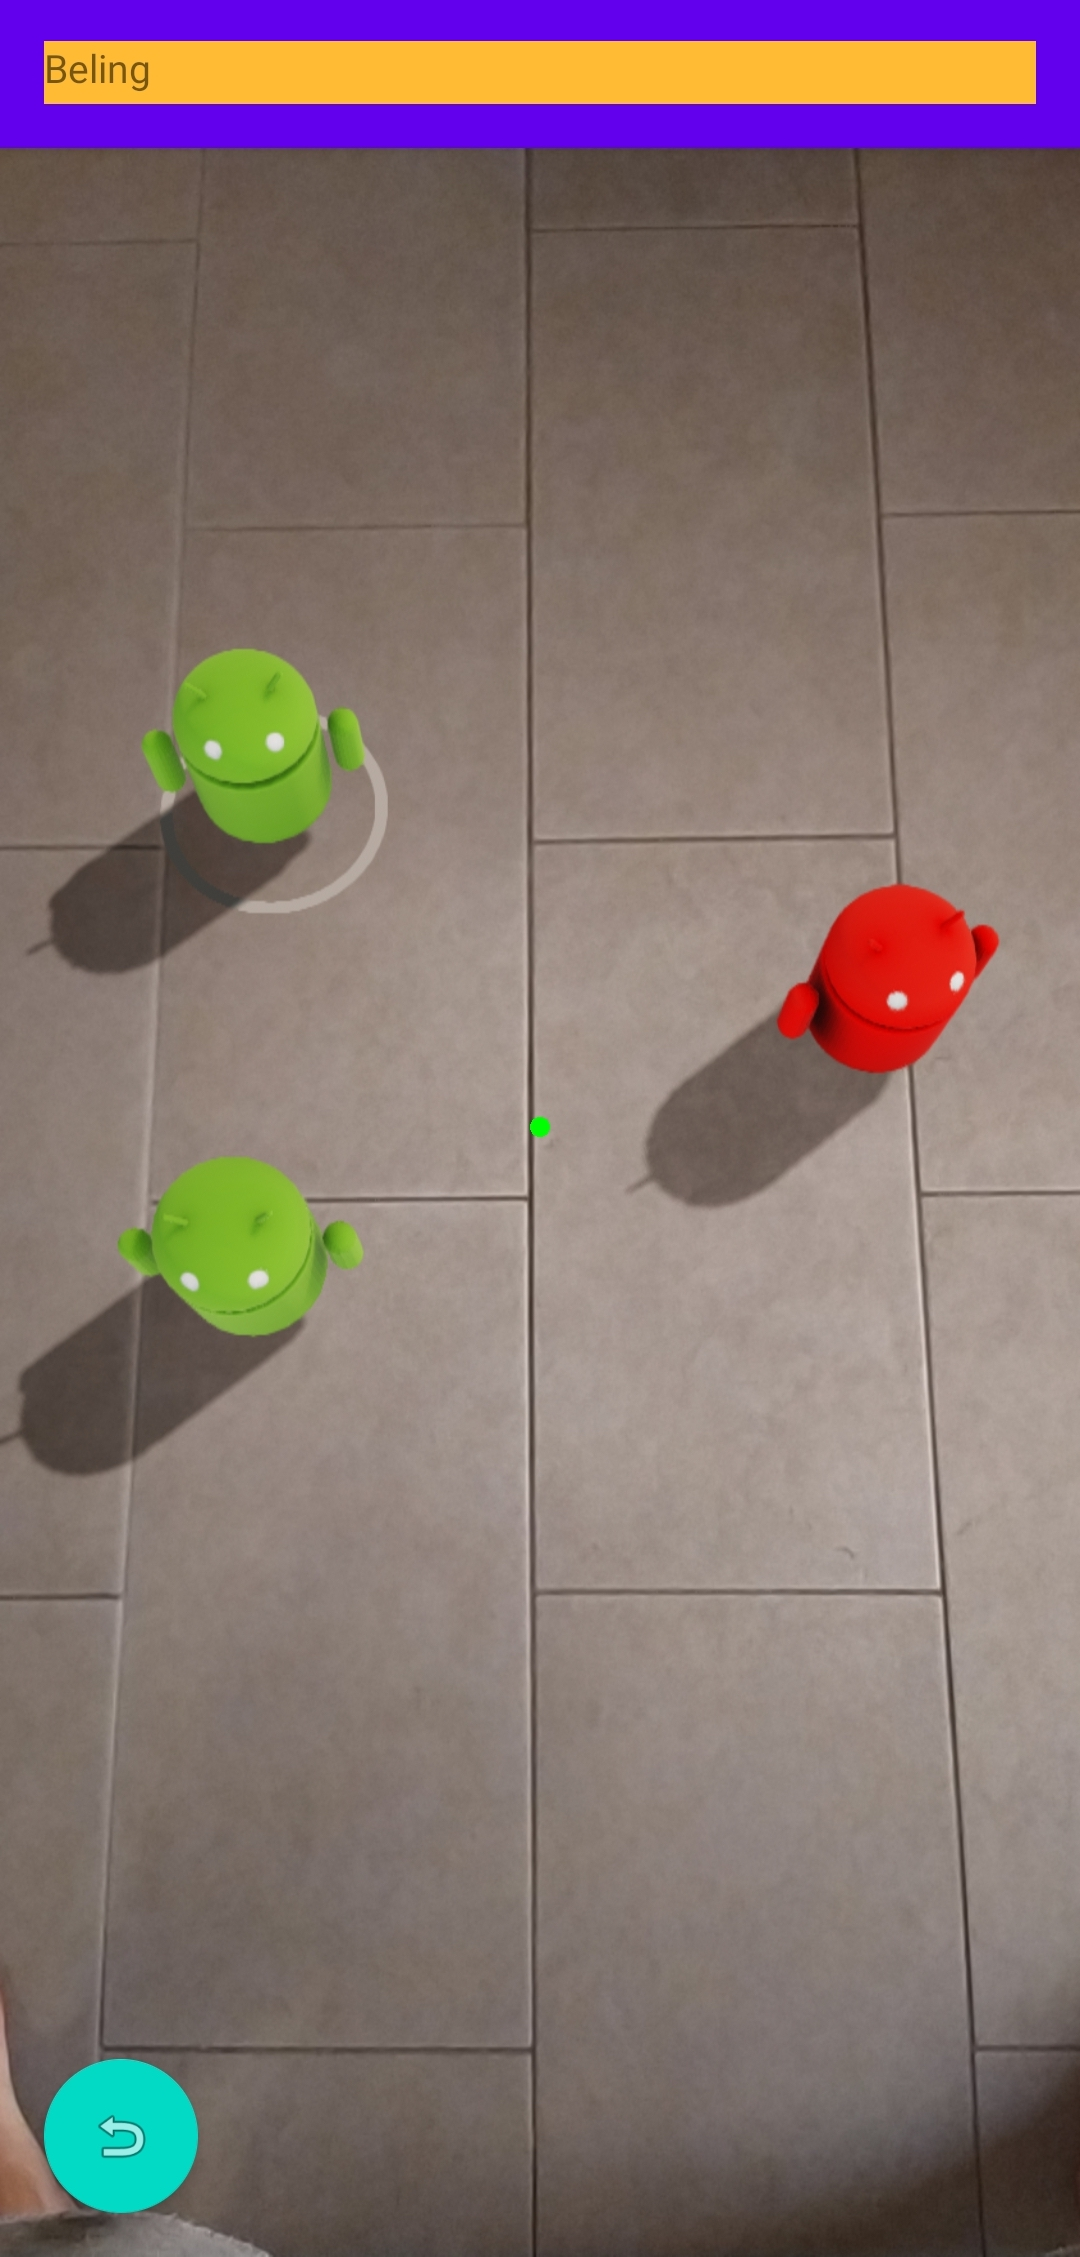
\includegraphics[width=10cm,height=7.5cm,keepaspectratio]{4Umsetzung/Bilder/show_objects_after_loading.jpg}
    \caption{Funktion Visualisierungs-Phase Teil 1}
    \label{pic:visual_objects}
\end{figure}
Eine weiter Funktion dieser Phase ist die Verwaltung der Objekte und deren Informationen. Wird ein Objekt anvisiert, kann über einen Klick auf das Objekt 
deren Informationen über ein PopUp angezeigt werden. Dieses beinhaltet den Namen des Objekts, den Status und die ID, die zu Anfang automatisch generiert 
und vergeben wurde. So kann zu jedem einzelnen Objekt, ohne großen Aufwand, dessen Informationen zur Verfügung gestellt werden. 
\begin{figure}[hbt!]
    \centering
    \subfigure[Anzeige der Objektinformationen 1]{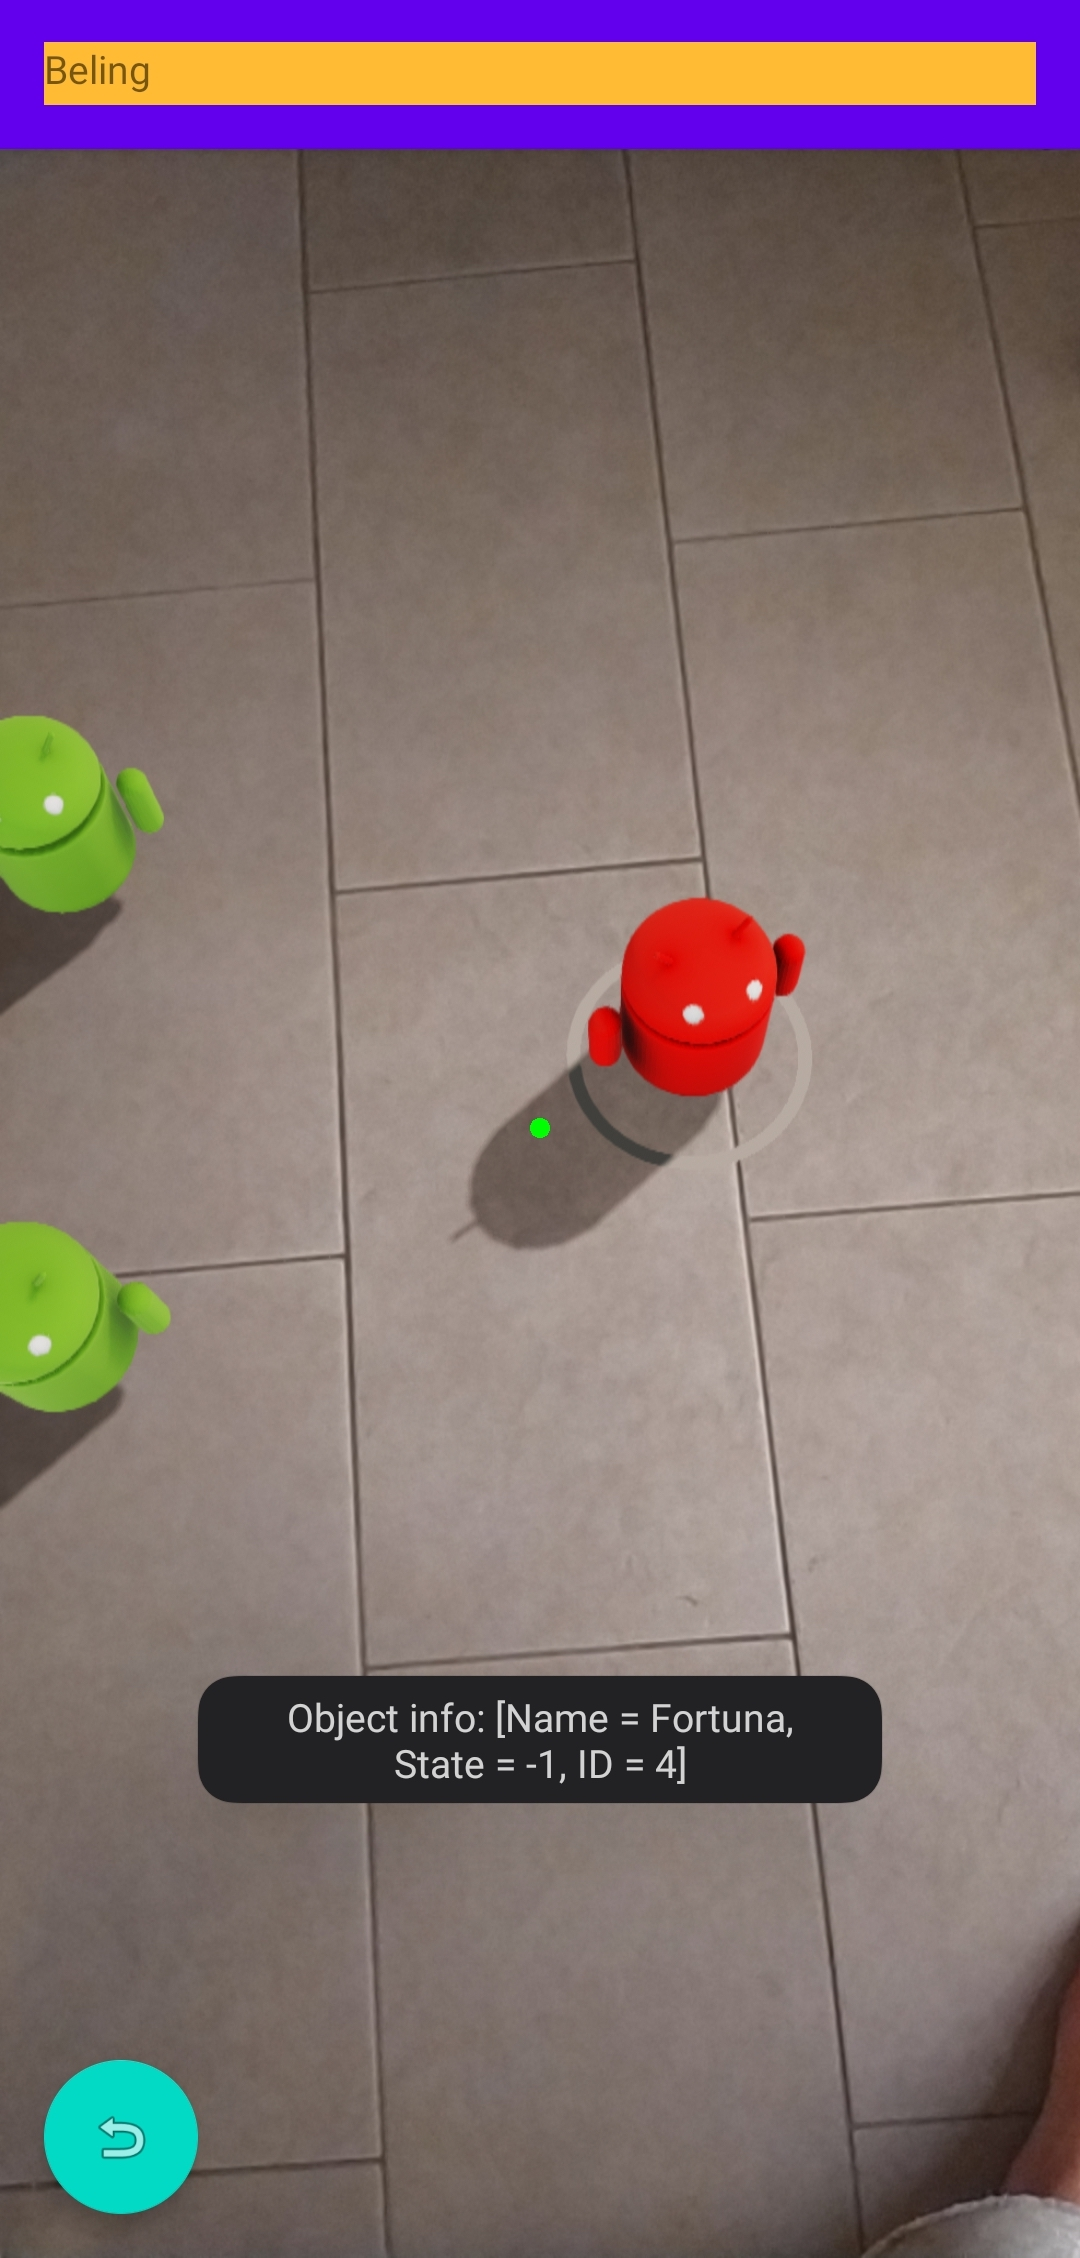
\includegraphics[width=10cm,height=7.5cm,keepaspectratio]{4Umsetzung//Bilder/show_data_to_obj_1.jpg}}
    \subfigure[Anzeige der Objektinformationen 2]{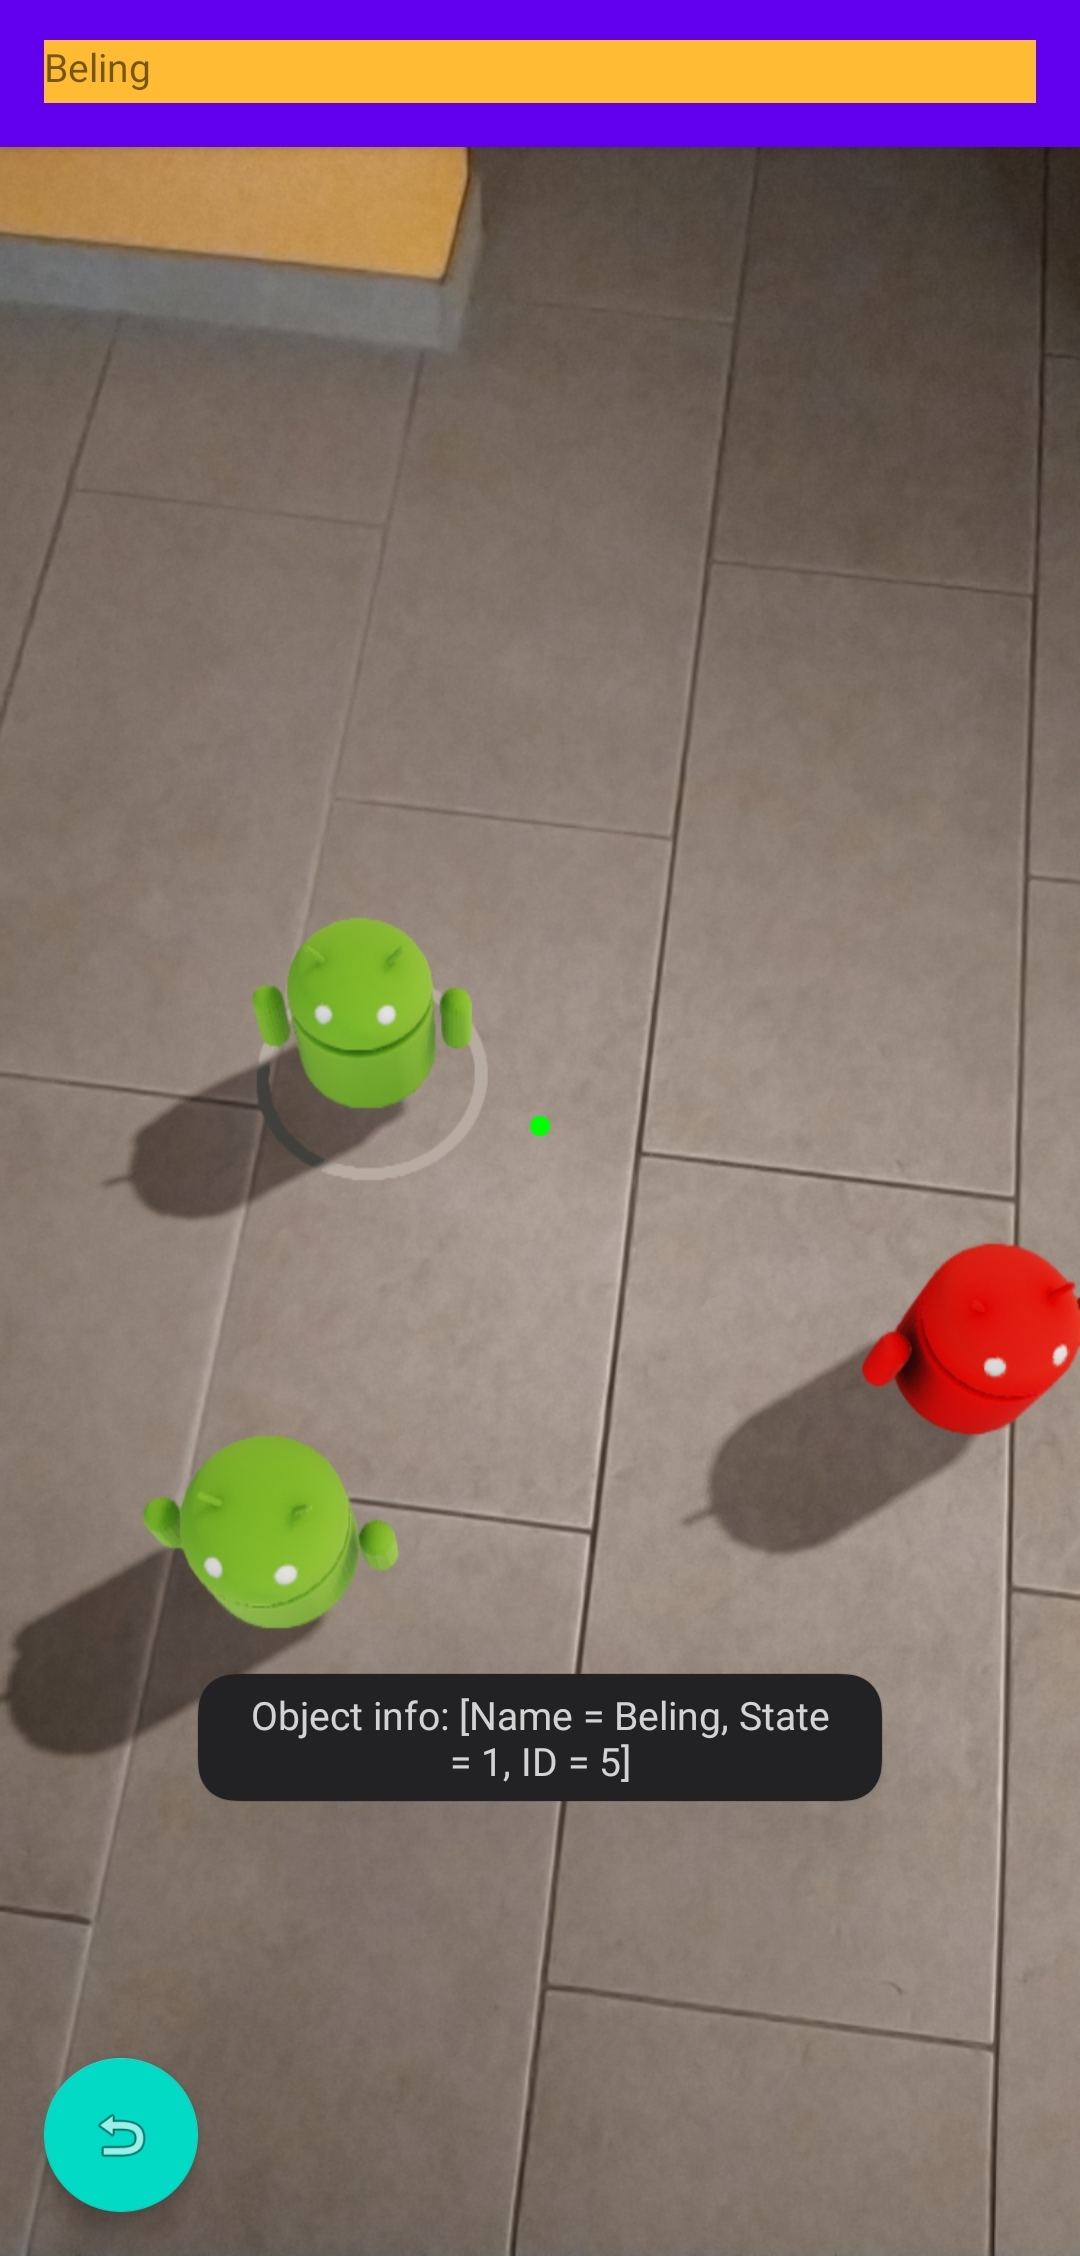
\includegraphics[width=10cm,height=7.5cm,keepaspectratio]{4Umsetzung/Bilder/show_data_to_obj_2.jpg}}
    \subfigure[Anzeige der Objektinformationen 3]{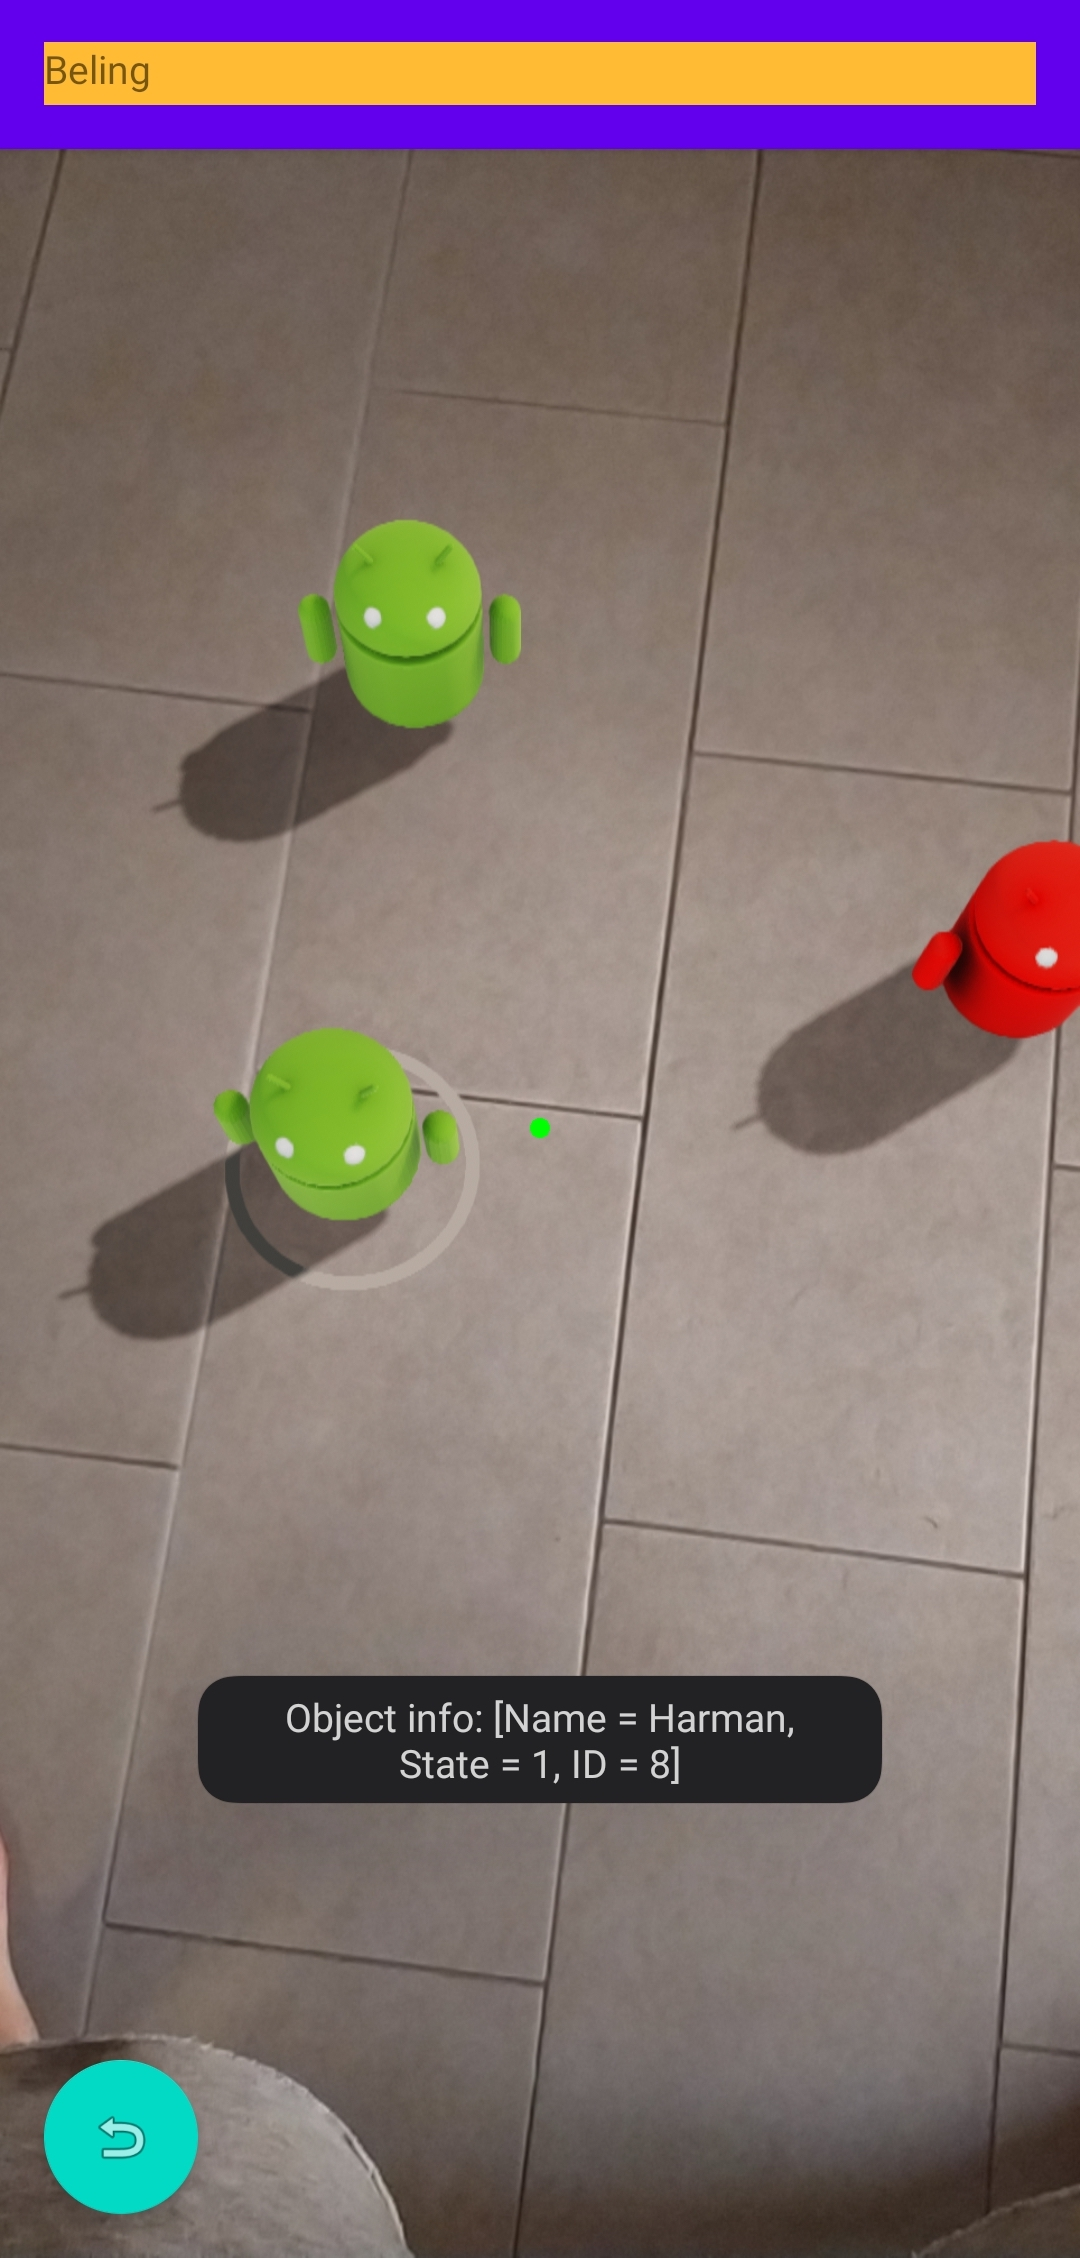
\includegraphics[width=10cm,height=7.5cm,keepaspectratio]{4Umsetzung/Bilder/show_data_to_obj_3.jpg}}
    \caption{Funktion Visualisierungs-Phase Teil 2}
    \label{pic:showdatatoobj}
\end{figure}
\pagebreak 
\\ 
\linebreak
Nachdem die einzelnen Aspekte der Front- und Backend-Entwicklung der drei Use Cases geschildert und so erfolgreich Einblicke in die Entwicklung, in 
aufgetretenen Hindernissen und Problemstellungen gewährleistet wurden, geht es nun mit der Evaluierung des Systems, dem Fazit und dem Ausblick weiter.

%werden die implementierten Funktionen anhand eines Testdurchlaufs nochmals genauer 
%dargelegt.
%\section{Testdurchlauf} %/ Test-Szenario
%\label{chap:testdurchlauf}
%Ergänzend zur Implementierung wird in diesem Abschnitt das Resultat und die Anwendung der Applikation anhand eines unabhängigen Tests praktiziert, um die 
%Erzeugnisse der Entwicklung darzustellen und gegebenenfalls erweiternd zur eigentlichen Entwicklungsbeschreibung Ergebnisse zu präsentieren.